%==============================================================================
%  ML Through the Looking Glass — Project presentation (~18 min, demo-forward)
%  Author: Alexandre Noel.  Supervisor: Prof. Nicolas Wu.  Imperial College London.
%
%  Build:        latexmk -pdf slides.tex     (or: pdflatex slides.tex  x2)
%  Speaker notes: uncomment the \setbeameroption line below to print notes pages.

%==============================================================================
\documentclass[aspectratio=169,11pt]{beamer}

\usetheme{default}
\usecolortheme{default}
\setbeamertemplate{navigation symbols}{}
\setbeamertemplate{footline}[frame number]
\setbeamertemplate{itemize items}[circle]

% --- Speaker notes (uncomment ONE to render notes) ---------------------------
% \setbeameroption{show notes}
% \setbeameroption{show notes on second screen=right}

% --- Fonts / encoding --------------------------------------------------------
\usepackage[T1]{fontenc}
\usepackage[utf8]{inputenc}
\usepackage{lmodern}
\usepackage{amsmath,amssymb}
\usepackage{booktabs}
\usepackage{listings}

% --- Imperial-ish palette ----------------------------------------------------
\definecolor{imperialblue}{RGB}{0,62,116}
\definecolor{imperiallight}{RGB}{0,110,175}
\definecolor{accent}{RGB}{198,12,48}
\definecolor{good}{RGB}{0,128,72}
\definecolor{codebg}{RGB}{245,245,245}

\setbeamercolor{structure}{fg=imperialblue}
\setbeamercolor{frametitle}{fg=imperialblue}
\setbeamercolor{title}{fg=imperialblue}
\setbeamercolor{section in toc}{fg=imperialblue}
\setbeamerfont{frametitle}{series=\bfseries}
\setbeamerfont{title}{series=\bfseries}
\setbeamerfont{footnote}{size=\tiny}
\setbeamercolor{footnote}{fg=black!60}
\setbeamercolor{footnote mark}{fg=imperiallight}
\renewcommand*{\footnoterule}{\vspace*{2pt}\hrule width 3cm height 0.3pt\vspace*{2pt}}

% --- Diagrams (reuse the thesis wire-diagram styles) -------------------------
\usepackage{tikz}
\usetikzlibrary{positioning, arrows.meta, calc, fit}
\tikzset{
  paralens/.style={draw, thick, minimum width=1.4cm, minimum height=0.9cm},
  wire/.style={->, >=Stealth, thick},
  inwire/.style={->, >=Stealth, semithick, gray!70!black}
}

% --- Where to find the (already-generated) training plots --------------------
\graphicspath{{../thesis/}{../thesis/figures/}{figures/}}

% --- Code listing style (ASCII only inside listings) -------------------------
\lstset{
  basicstyle=\ttfamily\small,
  backgroundcolor=\color{codebg},
  keywordstyle=\color{imperialblue}\bfseries,
  commentstyle=\color{good}\itshape,
  showstringspaces=false,
  columns=fullflexible,
  breaklines=true,
  frame=single,
  framesep=4pt,
  rulecolor=\color{gray!40},
  xleftmargin=4pt, xrightmargin=4pt,
}
\lstdefinelanguage{hs}{
  keywords={type,data,forall,Functor,Lens,ParaLens,Tensor,where,instance,class},
  morecomment=[l]{--},
  sensitive=true,
}

\title{ML Through the Looking Glass}
\subtitle{Machine Learning with Lenses in Haskell}
\author{Alexandre Noel}
\institute{Imperial College London \quad\textbar\quad Supervisor: Prof.\ Nicolas Wu}
\date{MEng Computing (AI \& ML)}

%==============================================================================
\begin{document}

%--- 1. TITLE -----------------------------------------------------------------
\begin{frame}[plain]
  \titlepage
  \begin{center}
    \footnotesize\color{imperialblue}
    A statically typed Haskell library for gradient-based learning, built out of optics.
  \end{center}
\end{frame}


%--- 2. THE PROBLEM -----------------------------------------------------------
\begin{frame}{How ML libraries train a model today}
  \begin{columns}[T]
    \begin{column}{0.54\textwidth}
      \centering
      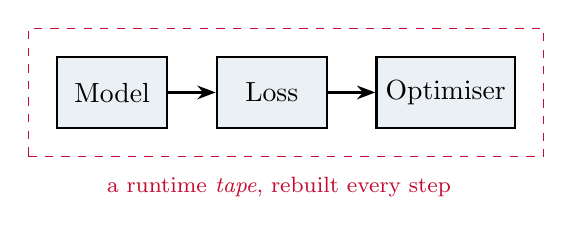
\begin{tikzpicture}[node distance=6mm]
        \node[paralens, fill=imperialblue!8] (m) {Model};
        \node[paralens, fill=imperialblue!8, right=of m] (l) {Loss};
        \node[paralens, fill=imperialblue!8, right=of l] (o) {Optimiser};
        \draw[wire] (m) -- (l); \draw[wire] (l) -- (o);
        \node[draw, dashed, accent, fit=(m)(l)(o), inner sep=10pt] {};
        \node[accent] at ($(m)!0.5!(o)+(0,-1.2)$) {\footnotesize a runtime \emph{tape}, rebuilt every step};
      \end{tikzpicture}

      \vspace{1em}
      \footnotesize
      Three separate components, wired together by hand. The gradients come from a
      \emph{tape}: every operation is recorded at runtime, then replayed in reverse.\footnote[frame]{Reverse-mode automatic differentiation, as in PyTorch: Paszke et al., NeurIPS 2019.}
    \end{column}
    \begin{column}{0.46\textwidth}
      \small This is convenient, but it has two costs.
      \begin{enumerate}\small\setlength\itemsep{0.4em}
        \item The tape is rebuilt on every step, so every step pays for graph allocation
              and dispatch.
        \item Shapes are only checked when a kernel runs, so a wrong shape crashes
              part-way through training:
      \end{enumerate}
      \vspace{0.4em}
      {\scriptsize\color{accent}
      \texttt{RuntimeError: mat1 and mat2 shapes}\\
      \texttt{cannot be multiplied (8x10 and 4x3)}}
    \end{column}
  \end{columns}
\end{frame}


%--- 3. THE QUESTION ----------------------------------------------------------
\begin{frame}{What if the model, the loss and the optimiser were one kind of object?}
  \begin{itemize}\setlength\itemsep{0.6em}
    \item A layer, a loss and an optimiser could all be the same composable thing.
    \item The chain rule could be nothing more than composing those things.
    \item And the whole abstraction could be checked for correctness, then compiled away.
  \end{itemize}
  \vspace{1em}
  \begin{block}{The question this thesis asks}
    The framework is Cruttwell et al.'s (2021)\footnote[frame]{Cruttwell, Gavranovi\'c, Ghani, Wilson \& Zanasi. \emph{Categorical Foundations of Gradient-Based Learning}. arXiv:2103.01931, 2021.}: category theory, with a dynamically-typed Python
    PoC. The question is: can we make the pure approach pay in a real language? That is, give up automatic differentiation and gain: speed, no abstraction overhead, and architectural mistakes caught at compile time. At what cost to expressiveness?
  \end{block}
\end{frame}


%--- 4. THE VIEW-UPDATE PROBLEM (intro) ---------------------------------------
\begin{frame}[fragile]{A lens solves the view--update problem}
  \small How do you read one part of a structure, and put a modified part back? A \emph{lens} bundles
  both as one value --- here the simplest, same-type variant:
\begin{lstlisting}[language=hs,basicstyle=\ttfamily\footnotesize]
data Lens' s a = Lens' { view :: s -> a, update :: s -> a -> s }
\end{lstlisting}
  \begin{columns}[T]
    \begin{column}{0.55\textwidth}
      \footnotesize Focus on the phone number inside an account:
\begin{lstlisting}[language=hs,basicstyle=\ttfamily\scriptsize]
newtype PhoneNumber = PhoneNumber Int
data Account = Account
  { phone :: PhoneNumber, accountId :: Int }

acctToPhone :: Lens' Account PhoneNumber
acctToPhone = Lens' phone
                    (\acc n -> acc{ phone = n })
\end{lstlisting}
    \end{column}
    \begin{column}{0.45\textwidth}
      \centering
      \resizebox{\textwidth}{!}{%
      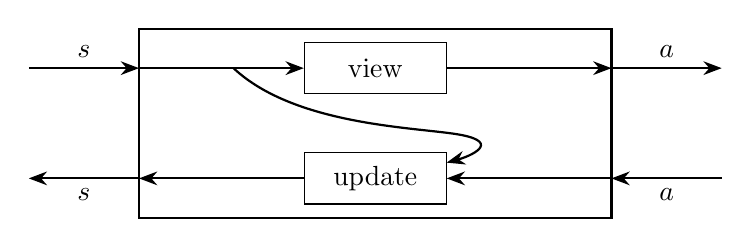
\begin{tikzpicture}
        \draw[thick] (-3,-1.2) rectangle (3,1.2);
        \node[draw, minimum width=1.8cm, minimum height=0.65cm] (f)  at (0,  0.7) {view};
        \node[draw, minimum width=1.8cm, minimum height=0.65cm] (fs) at (0, -0.7) {update};
        \coordinate (fork) at (-1.8, 0.7);
        \draw[wire] (-4.4,  0.7) -- node[above] {$s$}  (-3, 0.7);
        \draw[thick] (-3, 0.7) -- (fork);
        \draw[wire] (fork) -- (f.west);
        \draw[wire] (fork) .. controls (-1.0,-0.05) and (0.6,-0.05) .. (1.1,-0.15)
                    .. controls (1.6,-0.25) and (1.2,-0.42) .. ($(fs.east)+(0,0.2)$);
        \draw[wire] (f.east) -- (3, 0.7);
        \draw[wire] (3,  0.7) -- node[above] {$a$}  (4.4, 0.7);
        \draw[wire] (4.4, -0.7) -- node[below] {$a$} (3, -0.7);
        \draw[wire] (3, -0.7) -- (fs.east);
        \draw[wire] (fs.west) -- (-3, -0.7);
        \draw[wire] (-3,-0.7) -- node[below] {$s$} (-4.4, -0.7);
      \end{tikzpicture}}

      {\scriptsize \emph{view} runs forward ($s\!\to\!a$); \emph{update} runs backward and needs the
      original $s$, so the wire forks. ($s=$ Account, $a=$ Phone.)}
    \end{column}
  \end{columns}
\end{frame}


%--- 4b. VAN LAARHOVEN + TYPE-CHANGING ----------------------------------------
\begin{frame}{One function for both directions --- and it composes}
  \small Rather than store \texttt{view} and \texttt{update} separately, the van Laarhoven\footnote[frame]{The van Laarhoven / profunctor-optics encoding: Pickering, Gibbons \& Wu, \emph{Profunctor Optics}, 2017; Kmett's \texttt{lens} library.} encoding fuses both directions into a single higher-order function:
  \begin{center}\resizebox{0.82\linewidth}{!}{$
    \texttt{Lens s t a b} = \forall f.\ \mathrm{Functor}\,f \Rightarrow (a \to f\,b)\to s \to f\,t
  $}\end{center}
  \vspace{0.4em}
  \begin{columns}[T]
    \begin{column}{0.5\textwidth}
      \footnotesize
      \textbf{Both directions, from one function.} $f=\textsf{Const}$ recovers the read (view);
      $f=\textsf{Identity}$ recovers the write (update).
      \vspace{0.5em}

      \textbf{It composes for free.} A lens is just a function in continuation passing style, so two lenses compose with ordinary
      $(\circ)$ --- \texttt{outer\,.\,inner} --- no glue. (This is what later collapses the whole stack
      to direct calls.)
    \end{column}
    \begin{column}{0.5\textwidth}
      \footnotesize
      \textbf{Why four type variables}, not $s\!\to\!a\!\to\!s$? The value put back ($b$) and the
      result ($t$) may differ from what was read.
      \vspace{0.5em}

      On the next slide that difference is exactly a \emph{forward value} ($b$) versus a
      \emph{backward gradient} ($b'$) --- which a simple same-type lens could not express.
    \end{column}
  \end{columns}
\end{frame}


%--- 5. A PARAMETRIC LENS IS A LAYER -----------------------------------------
\begin{frame}{A layer is a lens that also carries parameters}
  \begin{columns}[T]
    \begin{column}{0.5\textwidth}
      \small
      A layer reads its weights going forward and updates them coming back, so we give the
      parameters a wire of their own:
      \begin{center}\resizebox{\linewidth}{!}{$\texttt{ParaLens p p' a a' b b' = Lens (p,a) (p',a') b b'}$}\end{center}
      \begin{itemize}\footnotesize
        \item $p,p'$ — parameters in and out
        \item $a,a'$ — data forward, gradient back
        \item $b,b'$ — output forward, gradient in
      \end{itemize}
      \vspace{0.3em}
      \footnotesize The forward and backward passes sit in the same value, written and type-checked
      together. The primed (gradient) types can differ from the forward ones --- this is why we needed the
      type-changing lens from the last slide.
    \end{column}
    \begin{column}{0.5\textwidth}
      \centering
      \resizebox{0.95\textwidth}{!}{%
      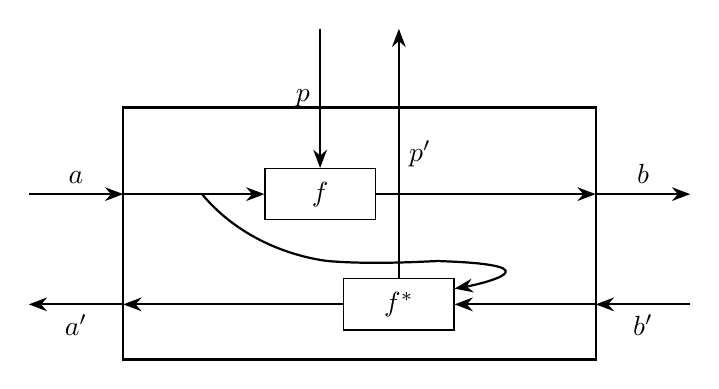
\begin{tikzpicture}
        \draw[thick] (-3,-1.4) rectangle (3,1.8);
        \node[draw, minimum width=1.4cm, minimum height=0.65cm] (f)  at (-0.5,  0.7) {$f$};
        \node[draw, minimum width=1.4cm, minimum height=0.65cm] (fs) at ( 0.5, -0.7) {$f^*$};
        \coordinate (fork) at (-2.0, 0.7);
        \draw[wire] (fs.north) -- node[right] {$p'$} (0.5, 2.8);
        \draw[wire] (-4.2,  0.7) -- node[above] {$a$}  (-3, 0.7);
        \draw[thick] (-3, 0.7) -- (fork);
        \draw[wire] (fork) -- (f.west);
        \draw[wire] (f.east) -- (3, 0.7);
        \draw[wire] (3,  0.7) -- node[above] {$b$}  (4.2, 0.7);
        \draw[wire] (4.2, -0.7) -- node[below] {$b'$} (3, -0.7);
        \draw[wire] (3, -0.7) -- (fs.east);
        \draw[wire] (fs.west) -- (-3, -0.7);
        \draw[wire] (-3,-0.7) -- node[below] {$a'$} (-4.2, -0.7);
        \draw[wire] (fork) .. controls (-1.5, 0.1) and (-0.8,-0.1) .. (-0.4,-0.15)
                    .. controls (0.2,-0.2) and (0.9,-0.15) .. (1.0,-0.15)
                    .. controls (2.6,-0.2) and (1.5,-0.45) .. ($(fs.east)+(0,0.2)$);
        \draw[wire] (-0.5, 2.8) -- node[left] {$p$} (f.north);
      \end{tikzpicture}}

      {\footnotesize parameters $p\!\to\!p'$ on the vertical wire; data $a\!\to\!b$ horizontal.}
    \end{column}
  \end{columns}
\end{frame}


%--- 6. COMPOSITION IS THE CHAIN RULE ----------------------------------------
\begin{frame}{Composing two lenses gives the chain rule, and infers the combined parameters}
  \centering
  \resizebox{0.92\textwidth}{!}{%
  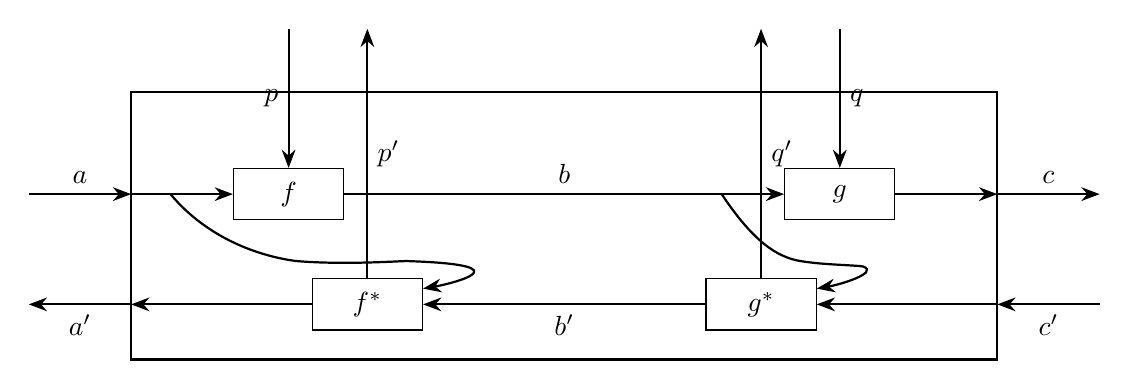
\begin{tikzpicture}
    \draw[thick] (-5.5,-1.4) rectangle (5.5,2.0);
    \node[draw, minimum width=1.4cm, minimum height=0.65cm] (f)  at (-3.5,  0.7) {$f$};
    \node[draw, minimum width=1.4cm, minimum height=0.65cm] (fs) at (-2.5, -0.7) {$f^*$};
    \node[draw, minimum width=1.4cm, minimum height=0.65cm] (g)  at ( 3.5,  0.7) {$g$};
    \node[draw, minimum width=1.4cm, minimum height=0.65cm] (gs) at ( 2.5, -0.7) {$g^*$};
    \draw[wire] (fs.north) -- node[right] {$p'$} (-2.5, 2.8);
    \draw[wire] (gs.north) -- node[right] {$q'$} ( 2.5, 2.8);
    \draw[wire] (-6.8,  0.7) -- node[above] {$a$}  (-5.5,  0.7);
    \draw[wire] (-5.5,  0.7) -- (f.west);
    \draw[wire] (g.east) -- (5.5,  0.7);
    \draw[wire] (5.5,   0.7) -- node[above] {$c$}  (6.8,  0.7);
    \draw[wire] (6.8,  -0.7) -- node[below] {$c'$} (5.5, -0.7);
    \draw[wire] (5.5,  -0.7) -- (gs.east);
    \draw[wire] (fs.west) -- (-5.5, -0.7);
    \draw[wire] (-5.5, -0.7) -- node[below] {$a'$} (-6.8, -0.7);
    \draw[wire] (f.east)  -- node[above] {$b$}  (g.west);
    \draw[wire] (gs.west) -- node[below] {$b'$} (fs.east);
    %% memorised forward branches: a copies into f*, b copies into g* (the backward
    %% passes need their original forward inputs), mirroring the single-lens diagram.
    \draw[wire] (-5.0, 0.7) .. controls (-4.5, 0.1) and (-3.8,-0.1) .. (-3.4,-0.15)
                .. controls (-2.8,-0.2) and (-2.1,-0.15) .. (-2.0,-0.15)
                .. controls (-0.4,-0.2) and (-1.5,-0.45) .. ($(fs.east)+(0,0.2)$);
    \draw[wire] ( 2.0, 0.7) .. controls ( 2.4, 0.1) and ( 2.7,-0.1)  .. ( 3.0,-0.15)
                .. controls ( 3.3,-0.2) and ( 3.7,-0.2)  .. ( 3.8,-0.22)
                .. controls ( 4.0,-0.3) and ( 3.5,-0.45) .. ($(gs.east)+(0,0.2)$);
    \draw[wire] (-3.5, 2.8) -- node[left]  {$p$} (f.north);
    \draw[wire] ( 3.5, 2.8) -- node[right] {$q$} (g.north);
  \end{tikzpicture}}

  \vspace{0.4em}
  \resizebox{\textwidth}{!}{$(\bullet)\ ::\ \texttt{ParaLens p p' a a' b b'}\ \to\
     \texttt{ParaLens q q' b b' c c'}\ \to\ \texttt{ParaLens (p,q) (p',q') a a' c c'}$}

  {\small Each layer only defines its own backward pass. Composition assembles the global chain
  rule, and the combined parameter type $(p,q)$ can be inferred rather than written out.}
\end{frame}


%--- 7. PIPELINE AS LENSES ----------------------------------------------------
\begin{frame}[fragile]{Every part of the training loop is the same object}
  \begin{columns}[T]
    \begin{column}{0.56\textwidth}
      \footnotesize
      \begin{itemize}\setlength\itemsep{0.35em}
        \item A \textbf{layer} is a parametric lens: forward output, backward gradient.
              \hfill{\scriptsize\color{gray}\texttt{ParaLens' p a b}}
        \item A \textbf{loss} is a lens too: forward it outputs the scalar loss; backward it takes the
              learning rate as the gradient seed. Its parameter is the target.
              \hfill{\scriptsize\color{gray}\texttt{ParaLens' t pred (t[])}}
        \item The \textbf{learning rate} is the \emph{cap} that closes that scalar to the unit
              \texttt{()} --- forward discards it, backward injects $-\eta$.
              \hfill{\scriptsize\color{gray}\texttt{LRLens}}
        \item An \textbf{optimiser} is a lens too: it reparametrises the parameter wire
              (\texttt{momentum}, \texttt{adam}) via \texttt{repara}.
              \hfill{\scriptsize\color{gray}\texttt{Lens' p p}}
      \end{itemize}
      \vspace{0.5em}
      So one whole training step is a single composed lens, and its backward pass \emph{is} the
      parameter update.
    \end{column}
    \begin{column}{0.44\textwidth}
      \centering
      \resizebox{\linewidth}{!}{%
      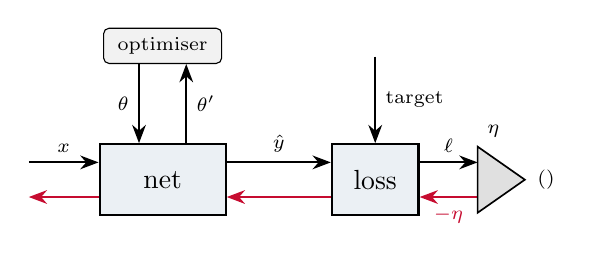
\begin{tikzpicture}
        \node[paralens, fill=imperialblue!8, minimum width=1.6cm] (net) at (0,0) {net};
        \node[paralens, fill=imperialblue!8, minimum width=1.1cm] (loss) at (2.7,0) {loss};
        \draw[wire] (-1.7,0.22) -- node[above]{\scriptsize$x$} ($(net.west)+(0,0.22)$);
        \draw[wire] ($(net.east)+(0,0.22)$) -- node[above]{\scriptsize$\hat y$} ($(loss.west)+(0,0.22)$);
        % forward: the scalar loss flows into the learning-rate cap, which closes it to the unit ()
        \draw[wire] ($(loss.east)+(0,0.22)$) -- node[above]{\scriptsize$\ell$} (4.0,0.22);
        \draw[wire, accent] (4.0,-0.22) -- node[below]{\scriptsize$-\eta$} ($(loss.east)+(0,-0.22)$);
        \fill[black!12, draw=black, semithick] (4.0,0.42) -- (4.0,-0.42) -- (4.6,0) -- cycle;
        \node[above] at (4.2,0.42) {\scriptsize$\eta$};
        \node[right=1pt] at (4.6,0) {\scriptsize$()$};
        \draw[wire, accent] ($(loss.west)+(0,-0.22)$) -- ($(net.east)+(0,-0.22)$);
        \draw[wire, accent] ($(net.west)+(0,-0.22)$) -- (-1.7,-0.22);
        \node[draw, rounded corners=2pt, fill=black!5, minimum width=1.5cm] (opt) at (0,1.7) {\scriptsize optimiser};
        \draw[wire] ($(opt.south)+(-0.3,0)$) -- node[left]{\scriptsize$\theta$} ($(net.north)+(-0.3,0)$);
        \draw[wire] ($(net.north)+(0.3,0)$) -- node[right]{\scriptsize$\theta'$} ($(opt.south)+(0.3,0)$);
        \draw[wire] ($(loss.north)+(0,1.1)$) -- node[right]{\scriptsize target} (loss.north);
      \end{tikzpicture}}

      \vspace{0.5em}
      {\scriptsize The \texttt{optimiser} box, at its simplest --- plain gradient descent:}
\begin{lstlisting}[language=hs,basicstyle=\ttfamily\scriptsize]
gradUpdate :: (Num p) => Lens' p p
gradUpdate = lens id (+)  -- read p; add gradient
\end{lstlisting}
    \end{column}
  \end{columns}
  \vspace{0.4em}
  \resizebox{\textwidth}{!}{$(\,\texttt{withGradDesc net}\ \bullet\ \texttt{loss}\,)\ \circ\ \texttt{lrSmooth}\;\eta
     \ ::\ \texttt{ParaLens' (params, target) input ()}$}
\end{frame}


%--- 8. WHY HASKELL -----------------------------------------------------------
\begin{frame}{Why build this in (4035 lines of) Haskell?}
  \begin{columns}[T]
    \begin{column}{0.33\textwidth}
      \begin{block}{\small The lens encoding}
        \footnotesize A lens is one function, and composing lenses is ordinary function
        composition. Once the functor is fixed at the call site, it optimises down to direct calls.
      \end{block}
      \begin{center}\footnotesize\color{imperiallight}no runtime overhead\end{center}
    \end{column}
    \begin{column}{0.33\textwidth}
      \begin{block}{\small Kind-level shapes (\texttt{DataKinds})}
        \footnotesize Shape and batch size are type-level naturals; \emph{type families} compute the
        conv/pool output shapes. An architectural mismatch does not type-check.
      \end{block}
      \begin{center}\footnotesize\color{imperiallight}shape errors at compile time\end{center}
    \end{column}
    \begin{column}{0.33\textwidth}
      \begin{block}{\small Device \& dtype, also in the type}
        \footnotesize \texttt{Tensor dv dt shape} carries the device (CPU/CUDA) and element type
        (Float/Double) too. One definition runs anywhere, switching is a one-line type application,
        and an invalid combination is a type error.
      \end{block}
      \begin{center}\footnotesize\color{imperiallight}one definition, any device \& precision\end{center}
    \end{column}
  \end{columns}
  % \vspace{0.8em}
  % \centering\small Three advantages from GHC's type system and the lens encoding --- the first two I'll show live.
\end{frame}


%--- 9. CONTRIBUTIONS BEYOND THE PAPER ----------------------------------------
\begin{frame}{What this work adds beyond the paper}
  \footnotesize The original is a small dynamically-typed Python proof of concept, storing each
  lens in an overhead-inducing data structure. This work combines the Cruttwell framework with the \emph{profunctor}
  (van Laarhoven) optics encoding, the combination behind our zero-cost result, and takes it well
  past where the paper stops:
  \begin{columns}[T]
    \begin{column}{0.48\textwidth}
      \begin{itemize}\footnotesize\setlength\itemsep{0.2em}
        \item \textbf{Static tensor types} (shape, batch, device, dtype) and \textbf{batching from the
              ground up}: vs the original's dynamic types, one example at a time.
        \item \textbf{Zero overhead, verified} by GHC Core.
        \item \textbf{Every backward pass machine-checked} to $10^{-4}$, which caught real gradient
              bugs the prototype had hidden.
        \item \textbf{Fixed two bugs in hasktorch's typed API} to make the conv backward pass
              type-check at all (Appendix A).
      \end{itemize}
    \end{column}
    \begin{column}{0.52\textwidth}
      \begin{itemize}\footnotesize\setlength\itemsep{0.25em}
        \item \textbf{Attention}, self- and multi-head\footnote[frame]{Attention: Vaswani et al., \emph{Attention Is All You Need}, NeurIPS 2017. Residual skips: He et al., \emph{Deep Residual Learning for Image Recognition}, CVPR 2016.} are the most complex derivation: a hand-written
              backward pass with the rank-one softmax Jacobian; head/embedding constraint enforced in the type.
        \item \textbf{Residual} skips as one combinator \texttt{skipPara}, where the identity gradient
              path \emph{falls out} of the structure naturally!
        \item \textbf{Autoencoders} (generative, not only discriminative); \textbf{type-level variable
              depth} (add a layer = one character).
      \end{itemize}
    \end{column}
  \end{columns}
  \vspace{0.4em}
  \centering{\scriptsize Validated on Iris (93\%), MNIST CNN (91\%, 1{,}527 params), residual MNIST, an
  autoencoder. Modest by design: the correctness evidence is the gradient tests, not the accuracy.}
\end{frame}


%==============================================================================
%  UNDER THE HOOD — code deep-dives (use spare time; skippable if running long)
%==============================================================================
\section{Under the hood}

%--- DD1: CORE + A LAYER ------------------------------------------------------
\begin{frame}[fragile]{Under the hood: the core is a handful of lines}
  \begin{columns}[T]
    \begin{column}{0.53\textwidth}
      \footnotesize The framework core --- the lens type, sequential composition $(\bullet)$, and the
      optimiser plug-in:
\begin{lstlisting}[language=hs,basicstyle=\ttfamily\scriptsize]
type ParaLens p p' a a' b b' = 
  Lens (p,a) (p',a') b b'
type ParaLens' p a b = Lens' (p,a) b

-- sequential composition
(.#.) :: ParaLens p p' a a' b b'
      -> ParaLens q q' b b' c c'
      -> ParaLens (p,q) (p',q') a a' c c'
ab .#. bc = swapFst . rotate
          . rightLens ab . bc

-- plug an optimiser onto the param wire
repara :: Lens q q' p p' 
       -> ParaLens p p' a a' b b' 
       -> ParaLens q q' a a' b b
repara r = (leftLens r .)
\end{lstlisting}
      % \scriptsize Composition combines the two parameter types automatically --- you never write the
      % plumbing.
    \end{column}
    \begin{column}{0.47\textwidth}
      \footnotesize A layer is a forward pass and its hand-derived backward, in one value:
\begin{lstlisting}[language=hs,basicstyle=\ttfamily\scriptsize]
linear = lens fwd rev where
  fwd (w, x) =
    matmul x (transp w)        -- x W^T
  rev (w, x) grad =
    ( matmul (transp grad) x   -- dL/dW
    , matmul grad w )          -- dL/dx
\end{lstlisting}
      \scriptsize Forward $xW^\top$; backward the two matrix-calculus gradients. \textit{(\texttt{T.}
      qualifiers elided.)}

      \vspace{0.4em}
      \footnotesize Compose it with the bias via $(\bullet)$ for a full affine layer, the combined
      parameter can be inferred:
\begin{lstlisting}[language=hs,basicstyle=\ttfamily\scriptsize]
-- param inferred as (W, b):
--   (t [o,i], t [o])
matMulLensCore = linear .#. addLens
\end{lstlisting}
    \end{column}
  \end{columns}
\end{frame}


%--- DD2: skipPara ------------------------------------------------------------
\begin{frame}[fragile]{Under the hood: residual connections in one line}
  \footnotesize A skip connection $y=f(x)+x$ is a single higher-order combinator, built from pieces
  that already exist:
\begin{lstlisting}[language=hs,basicstyle=\ttfamily\footnotesize]
splitIso = iso (join (,)) (uncurry (+))   -- fwd: duplicate;  bwd: sum

skipPara f = rightLens splitIso . from rotate . alongside f id . from splitIso
\end{lstlisting}
  \footnotesize \texttt{splitIso} fans the input into two copies going forward and \emph{sums} the two
  gradients coming back; \texttt{from splitIso} is its inverse. So the residual's identity gradient
  path \emph{is} that setter directly! One application is a residual
  block:
\begin{lstlisting}[language=hs,basicstyle=\ttfamily\footnotesize]
resBlock = skipPara (matMulLens . relu .#. matMulLens)
\end{lstlisting}
\end{frame}


%--- DD3: TYPE-LEVEL DEPTH ----------------------------------------------------
\begin{frame}[fragile]{Under the hood: depth-\texttt{n} networks by typeclass induction}
  \footnotesize Depth is a compile-time number. \texttt{Stack.hs} builds the network --- and its
  parameter type --- by induction over Peano naturals:
\begin{lstlisting}[language=hs,basicstyle=\ttfamily\scriptsize]
data PeanoNat = One | Succ PeanoNat

type family Stacked n m where           -- the parameter type: a nested tuple
  Stacked  One     m = m
  Stacked (Succ n) m = (m, Stacked n m)

class StackN n where
  stack :: ParaLens' p a a -> ParaLens' (Stacked n p) a a

instance StackN One                  where stack l = l
instance StackN n => StackN (Succ n) where
  stack l = l .#. stack @n l
  {-# INLINE stack #-}                  -- crucial: unrolls to zero-overhead Core
\end{lstlisting}
  \footnotesize At each $n$ the parameter type is a fully concrete nested tuple, so GHC unboxes it to
  the same Core as a hand-written $n$-layer network.
\end{frame}


%--- DD4: ATTENTION BACKWARD --------------------------------------------------
\begin{frame}[fragile]{Under the hood: the attention backward pass, by hand}
  \footnotesize The reverse pass for scaled dot-product attention: six weight/activation gradients
  and the softmax correction:
\begin{lstlisting}[language=hs,basicstyle=\ttfamily\scriptsize]
rev (p@(wq,wk,wv,wo), x) dOut = ((dWq,dWk,dWv,dWo), dX)
  where (q,k,v, weights, attn, _) = runFwd p x   -- recompute intermediates
        dAttn    = matmul dOut wo
        dWo      = wGrad attn dOut
        dWeights = mm dAttn (tr v)
        dV       = mm (tr weights) dAttn
        dScores  = softmaxBwd weights dWeights    -- the rank-one softmax Jacobian
        dQ = scale' (mm dScores k);  dK = scale' (mm (tr dScores) q)
        dWq = wGrad x dQ;  dWk = wGrad x dK;  dWv = wGrad x dV
        dX  = matmul dQ wq + matmul dK wk + matmul dV wv

softmaxBwd w dw = w * sub dw dot               -- Y * (dY - sum_j Y_j dY_j)
  where dot = reshape @[b,s,1] (sumDim @2 (w * dw))
\end{lstlisting}
  % \scriptsize The hardest derivation in the library --- and it is verified, not assumed.
  % \textit{(\texttt{T.} qualifiers elided.)}
\end{frame}


%==============================================================================
%  DEMO
%==============================================================================
\section{Demonstration}
\begin{frame}[plain]
  \centering
  \vfill
  {\Huge\bfseries\color{imperialblue} Demonstration}\\[1.2em]
  {\large\color{imperialblue} Three things to show:}\\[0.8em]
  \begin{minipage}{0.86\textwidth}\centering\small
    1.\ the compiler computes the tensor shapes and rejects a bad architecture\\[0.3em]
    2.\ the lens abstraction vanishes from the compiled code, even at variable depth\\[0.3em]
    3.\ it trains correctly, and faster than eager PyTorch
  \end{minipage}
  \vfill
\end{frame}


%--- DEMO 1: STATIC SIZING ----------------------------------------------------
\begin{frame}[fragile]{Demo, part 1: the compiler does the kernel-size arithmetic}
  \small Every spatial dimension in the MNIST CNN is \emph{computed} by a type family
  ($o=\lfloor(h-k+2p)/s\rfloor+1$), not written by hand:
\begin{lstlisting}[basicstyle=\ttfamily\footnotesize]
[b,1,28,28] --conv 3x3--> [b,3,26,26] --pool--> [b,3,13,13]
            --conv 4x4--> [b,5,10,10] --pool--> [b,5, 5, 5]
            --flatten--> [b,125] --dense 125->10--> [b,10]
\end{lstlisting}
  \footnotesize Change \texttt{conv1} from \texttt{3x3} to \texttt{4x4}: the compiler recomputes the
  whole chain, the second pool now yields \texttt{[5,4,4]} not \texttt{[5,5,5]}, and it stops compiling.
\begin{lstlisting}[basicstyle=\ttfamily\footnotesize,backgroundcolor=\color{accent!8},keywordstyle=\color{accent}]
  * Couldn't match type '4' with '5'
      (conv1=4x4 pools to [5,4,4], not the [5,5,5] flatten)
\end{lstlisting}
  \centering\footnotesize No intermediate sizes were specified. A wrong kernel is a type error,
  not a runtime crash.
\end{frame}


%--- DEMO 2: ZERO OVERHEAD + VARIABLE DEPTH -----------------------------------
\begin{frame}[fragile]{Demo, part 2: the abstraction vanishes, even at variable depth}
  \small One lens network vs a hand-written one: the \emph{same} optimised GHC Core worker.
\begin{lstlisting}[basicstyle=\ttfamily\scriptsize]
$s$wtranspose w1   $wmatmul_tt x W1^T   $wadd b1   $wsigmoid_t ...
$s$wtranspose w2   $wmatmul_tt h1 W2^T  $wadd b2   $wsigmoid      (8 calls, identical)
\end{lstlisting}
  \footnotesize The depth-\texttt{n} network is built by typeclass induction over Peano naturals
  (\texttt{Stack.hs}), yet the abstraction is still gone and the Core stays flat:
\begin{lstlisting}[basicstyle=\ttfamily\footnotesize]
$ grep -c 'ParaLens|repara|stack' Iris.dump-simpl     # at @20 and @50
  0
$ wc -l Iris.dump-simpl       # @20 -> 1800    @50 -> 4900   (~103/layer, linear)
\end{lstlisting}
  \centering\footnotesize \texttt{ParaLens}, $(\bullet)$, \texttt{repara}, the van Laarhoven
  $\forall f$: all absent at every depth. Adding a layer is a one-character change to \texttt{@n}.
\end{frame}


%--- DEMO 3: IT LEARNS + CORRECTNESS ------------------------------------------
\begin{frame}{Demo, part 3: it trains --- and the hand-derived gradients are checked}
  \begin{columns}[T]
    \begin{column}{0.58\textwidth}
      \centering
      
\includegraphics[width=\textwidth]{mnist_training.png}
      {\scriptsize MNIST CNN, 91.4\% on the 10k test set (1{,}527 params, 6k train).}
    \end{column}
    \begin{column}{0.42\textwidth}
      \footnotesize Correctness is not left to chance. Every hand-written backward pass is
      cross-checked against PyTorch autograd:
      \vspace{0.4em}

      {\ttfamily\footnotesize cabal test $\rightarrow$ 24/24 tests passed\\ \mbox{}\quad(max abs err $< 10^{-4}$)}

      \vspace{0.5em}
      including the \emph{conv kernel gradient} and the \emph{softmax Jacobian}, plus a full-epoch
      Iris equivalence test against a dynamic reference.
    \end{column}
  \end{columns}
\end{frame}


%--- DEMO 4: SPEED ------------------------------------------------------------
\begin{frame}{Demo, part 3 (cont.): faster than eager PyTorch, and why}
  \centering
  \begin{tabular}{@{}lrl@{}}
    \toprule
    Implementation (Iris MLP, CPU, per epoch) & Time & \\
    \midrule
    \textbf{typed lens}        & \textbf{689\,$\mu$s} & \\
    PyTorch eager (autograd)   & 3{,}631\,$\mu$s & {\color{good}\textbf{5.3$\times$ slower}} \\
    \bottomrule
  \end{tabular}

  {\scriptsize measured with Criterion\footnote[frame]{O'Sullivan, \texttt{criterion}: a Haskell micro-benchmarking library.}}

  \vspace{0.6em}
  \begin{minipage}{0.86\textwidth}\footnotesize
  There is no tape to build, and the hand-derived backward reduces to the \emph{same} LibTorch calls
  as the forward. Isolating the cost: building the autograd graph alone is $\sim$93\% of the baseline.
  The forward pass is within noise of a hand-rolled version (6.9 vs 6.8\,$\mu$s).
  \end{minipage}

  \vspace{0.8em}
  \centering\footnotesize \emph{But eager PyTorch is the soft baseline.} The honest comparison is JAX
  $\rightarrow$
\end{frame}


%==============================================================================
%  CLOSE
%==============================================================================
\section{Wrap-up}

%--- THE HONEST COMPARISON: JAX (promoted to main) ----------------------------
\begin{frame}{The honest comparison is JAX}
  \small JAX\footnote[frame]{Bradbury et al., \emph{JAX: composable transformations of Python+NumPy programs}, 2018; lowered through the XLA compiler.} also removes the per-step tape: \texttt{jit} traces once and XLA compiles a fused
  executable. At scale XLA's fusion will \emph{beat} this library (which calls kernels one at a time
  over FFI, no fusion). \textbf{The 5.3$\times$ is against eager PyTorch only, not a speed claim
  against JAX.} The real differences are elsewhere:
  \vspace{0.4em}
  \begin{center}\footnotesize
  \begin{tabular}{@{}lll@{}}
    \toprule
                   & \textbf{JAX} & \textbf{This work} \\
    \midrule
    Per-step tape  & removed (jit\,/\,XLA)        & removed (GHC inlining) \\
    Speed at scale & XLA fusion \textbf{(wins)}   & per-kernel FFI, no fusion \\
    Shape safety   & dynamic, at trace, per input & \textbf{static, compile-time, total} \\
    Mechanism      & tracer $\to$ jaxpr $\to$ XLA & general compiler, ordinary source \\
    Generality     & smooth real-valued autodiff  & \textbf{any CRDC} (real done; discrete open) \\
    \bottomrule
  \end{tabular}
  \end{center}
  \centering\footnotesize Against JAX the contribution is static safety, general-purpose erasure, and
  being parametric over the category, not raw speed.
\end{frame}


%--- 9. LIMITATIONS -----------------------------------------------------------
\begin{frame}{What it does not do}
  \begin{columns}[T]
    \begin{column}{0.5\textwidth}
      \footnotesize Boundaries of the current design:
      \begin{itemize}\footnotesize\setlength\itemsep{0.25em}
        \item Stateful or stochastic layers (dropout, batch-norm) do not fit a pure, deterministic lens.
        \item Global, step-dependent state has no home: Adam's bias correction needs a step counter,
              which I left out.
        \item Attention recomputes its forward pass in the backward; the lens type has no channel for
              cached activations (and GHC does not spot the duplication here).
      \end{itemize}
    \end{column}
    \begin{column}{0.5\textwidth}
      \footnotesize Costs of the approach:
      \begin{itemize}\footnotesize\setlength\itemsep{0.25em}
        \item Type errors can be hard to read; a shape mismatch can surface inside a
              \texttt{MonadReader} trace.
        \item The benchmark is small, CPU-only, and against eager PyTorch; JAX removes the tape too,
              so this is not a general speed claim.
        \item The guarantees need Haskell fluency to use.
      \end{itemize}
    \end{column}
  \end{columns}
  \vspace{0.4em}
  \centering\footnotesize Where the lens model stops, and the agenda for what comes next.
\end{frame}


%--- 10. WIDER VALUE + CLOSE --------------------------------------------------
\begin{frame}{Where the value is}
  \begin{itemize}\setlength\itemsep{0.5em}
    \item Whole classes of configuration mistakes, wrong shapes, wrong device, wrong depth, move
          from runtime failures to compile errors. Porting the untyped prototype to types actually
          surfaced gradient bugs that equal-dimension tests had hidden.
    \item It is a working and efficient instance of the categorical account of learning, rather than
          only a paper.
    \item Next steps: discrete and probabilistic CRDCs (learning beyond real vectors), 
          recurrence via \texttt{repara} on the state wire,
          improved inlining of fwd/bwd pass duplication (TTH?).
  \end{itemize}
  \vspace{0.8em}
  \begin{block}{}
    \centering In short: by writing the backward passes by hand and checking them, and by leaning on
    the type system and the optimiser, the library gets compile-time safety and no runtime overhead
    at once.
  \end{block}
  \vspace{0.4em}
  \centering\small Thank you for listening, and happy to take questions!
\end{frame}


%==============================================================================
%  BACKUP / Q&A SLIDES  (not part of the timed talk)
%==============================================================================
\appendix
\begin{frame}[plain]
  \centering\vfill
  {\Huge\bfseries\color{imperialblue} Backup slides}\\[0.6em]
  {\large for questions}
  \vfill
\end{frame}

\begin{frame}[fragile]{Backup: van Laarhoven, one function for both directions}
  \small Choosing the functor recovers each direction at no cost (\texttt{Const} and \texttt{Identity}
  erase via \texttt{coerce}\footnote[frame]{Safe, zero-cost coercions for Haskell: Breitner, Eisenberg, Peyton Jones \& Weirich, ICFP 2014.}):
\begin{lstlisting}[language=hs,basicstyle=\ttfamily\footnotesize]
type Lens s t a b = forall f. Functor f => (a -> f b) -> s -> f t
-- f = Const b  : fmap = flip const   => collapses to the getter (view)
-- f = Identity : fmap = coerce       => collapses to the setter (update)
\end{lstlisting}
  That is why composition is just $(\circ)$, and why GHC can inline the whole stack to direct calls.
\end{frame}

\begin{frame}{Backup: the softmax backward is a rank-one correction}
  For a row $y=\mathrm{softmax}(x)$ and incoming gradient $g$:
  \[ \frac{\partial L}{\partial x_i} \;=\; y_i\!\left(g_i - \sum_j y_j\,g_j\right). \]
  Hand-derived; the inner dot product is one \texttt{sumDim} along the class axis, broadcast back.
  This is the trickiest backward pass in the library, and it is cross-checked against autograd.
\end{frame}

\begin{frame}{Backup: why descent works, the CRDC natural addition}
  The training loop performs the categorical update\footnote[frame]{Cartesian Reverse Differential Categories: Cruttwell et al., arXiv:2103.01931, 2021.}
  \[ \theta_{\text{new}} \;=\; \theta_{\text{old}} + \partial\theta. \]
  $\partial\theta$ is whatever the backward pass emits; the sign and scale come from the learning-rate
  cap ($\alpha=-\eta$ gives descent, $\alpha>0$ gives ascent, e.g.\ DeepDream). The update rule itself
  never changes, and it works in any CRDC, not only Euclidean space.
\end{frame}

\begin{frame}{Backup: optimisers as lenses, per layer}
  \centering
  \resizebox{0.85\textwidth}{!}{%
  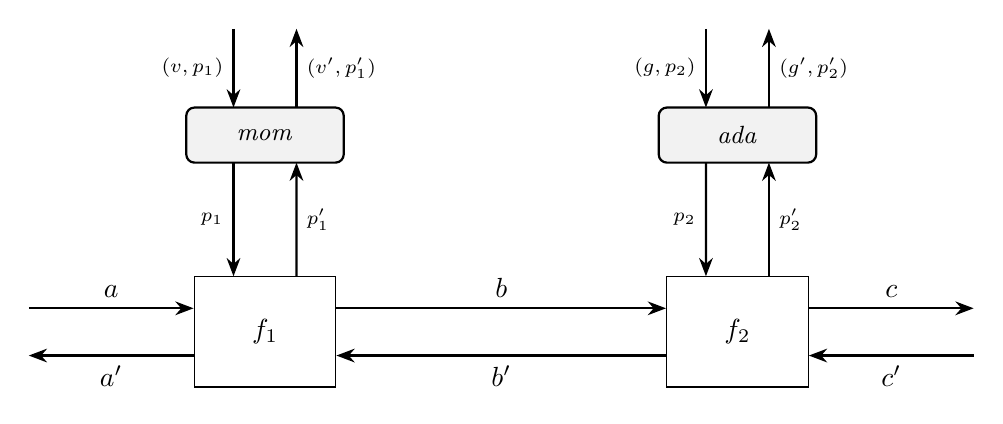
\begin{tikzpicture}
    \node[draw, minimum width=1.8cm, minimum height=1.4cm] (L1) at (-3, 0) {$f_1$};
    \node[draw, minimum width=1.8cm, minimum height=1.4cm] (L2) at ( 3, 0) {$f_2$};
    \node[draw, thick, fill=black!5, minimum width=2.0cm, minimum height=0.7cm,
          rounded corners=3pt] (mom) at (-3, 2.5) {\small$\mathit{mom}$};
    \node[draw, thick, fill=black!5, minimum width=2.0cm, minimum height=0.7cm,
          rounded corners=3pt] (ada) at ( 3, 2.5) {\small$\mathit{ada}$};
    \draw[wire] (-3.4, 3.85) -- node[left]  {\scriptsize$(v,p_1)$}   (-3.4, 2.85);
    \draw[wire] (-3.4, 2.15) -- node[left]  {\scriptsize$p_1$}        ($(L1.north)+(-0.4,0)$);
    \draw[wire] ($(L1.north)+(0.4,0)$) -- node[right] {\scriptsize$p_1'$}     (-2.6, 2.15);
    \draw[wire] (-2.6, 2.85) -- node[right] {\scriptsize$(v',p_1')$}  (-2.6, 3.85);
    \draw[wire] ( 2.6, 3.85) -- node[left]  {\scriptsize$(g,p_2)$}   ( 2.6, 2.85);
    \draw[wire] ( 2.6, 2.15) -- node[left]  {\scriptsize$p_2$}        ($(L2.north)+(-0.4,0)$);
    \draw[wire] ($(L2.north)+(0.4,0)$) -- node[right] {\scriptsize$p_2'$}     ( 3.4, 2.15);
    \draw[wire] ( 3.4, 2.85) -- node[right] {\scriptsize$(g',p_2')$}  ( 3.4, 3.85);
    \draw[wire] (-6, 0.3)  -- node[above] {$a$}  ($(L1.west)+(0, 0.3)$);
    \draw[wire] ($(L1.east)+(0, 0.3)$) -- node[above] {$b$} ($(L2.west)+(0, 0.3)$);
    \draw[wire] ($(L2.east)+(0, 0.3)$) -- node[above] {$c$} (6, 0.3);
    \draw[wire] ($(L1.west)+(0,-0.3)$) -- node[below] {$a'$} (-6, -0.3);
    \draw[wire] ($(L2.west)+(0,-0.3)$) -- node[below] {$b'$} ($(L1.east)+(0,-0.3)$);
    \draw[wire] (6, -0.3) -- node[below] {$c'$} ($(L2.east)+(0,-0.3)$);
  \end{tikzpicture}}

  \footnotesize $f_1$ uses momentum, $f_2$ uses AdaGrad\footnote[frame]{AdaGrad: Duchi, Hazan \& Singer, JMLR 2011. Adam: Kingma \& Ba, ICLR 2015.}: different optimiser state types on each
  vertical wire, assembled by $(\bullet)$, with no global optimiser object.
\end{frame}

\begin{frame}[fragile]{Backup: type-checker and Core scaling with depth}
  \small Depth is a compile-time \texttt{Nat}; \texttt{Stack.hs} builds the network by typeclass
  induction over Peano naturals:
\begin{lstlisting}[language=hs,basicstyle=\ttfamily\footnotesize]
net = runFullModel $ irisModel @20   -- 1,800 lines of Core
net = runFullModel $ irisModel @50   -- 4,900 lines of Core
\end{lstlisting}
  Core grows linearly, roughly 103 lines per layer, and the lens abstraction is absent at every depth.
  Adding a layer is a one-character change to \texttt{@n}.
\end{frame}

\begin{frame}{Backup: why not the \texttt{backprop} library?}
  \small A van Laarhoven lens is already a single function whose getter is the forward pass and whose
  setter is the gradient, encoded statically. \texttt{backprop}\footnote[frame]{Le, the \texttt{backprop} Haskell library (Hackage), 2018.}, like autograd, builds a runtime tape,
  which cannot be inlined away and brings back the overhead this design removes. The CRDC update
  $\theta\!\leftarrow\!\theta+\partial\theta$ is also defined for any category, including discrete ones,
  whereas \texttt{backprop} is tied to differentiable real-valued functions.
\end{frame}

\begin{frame}[fragile]{Backup: bugs found in hasktorch's typed API (Appendix A)}
  \small Getting the convolution backward pass to type-check meant fixing two bugs in the upstream
  typed bindings\footnote[frame]{hasktorch: typed Haskell bindings to LibTorch, the PyTorch C++ backend.} (hasktorch 0.2, LibTorch 2.x):
  \begin{itemize}\footnotesize\setlength\itemsep{0.4em}
    \item \texttt{convTranspose2d} applied the \texttt{ConvSideCheck} constraint with the input and
          output spatial sizes \emph{swapped}. Invisible for 1$\times$1 kernels (the only case the
          upstream test suite exercised); for every other kernel it rejected valid calls and accepted
          invalid ones.
    \item \texttt{im2col}'s binding type-checked but threw at runtime: its \texttt{Castable} instance
          delegated to an unimplemented \texttt{makeTuple2}. Fixed by casting each pair through a
          two-element list instead.
  \end{itemize}
  Both surfaced only by pushing the typed API past where it had been exercised --- and both are worked
  around in \texttt{Static/Bugfix.hs}, verified against dynamic calls.
\end{frame}

\end{document}
